\documentclass[10pt,a4paper]{article}

\usepackage[latin1]{inputenc}
\usepackage{amsmath}
\usepackage{amsfonts}
\usepackage{amssymb}
\usepackage{graphicx}
\usepackage{listings}
\title{Assignment No :A2}
\date{}

\begin{document}
\maketitle
\section{Title:}
Concurrent quick sort

\section{Problem Definition}
Using Divide and Conquer Strategies to design an efficient class for Concurrent Quick Sort and the input data is stored using XML. Use object oriented software design method and Modelio/ StarUML2.x Tool.
Perform the efficiency comparison with any two software design methods. Use necessary USE-CASE
diagrams and justify its use with the help of mathematical modeling. Implement the design using Scala/
Python/Java/C++.

\section{Learning Objectives}
\begin{enumerate}
\item To understand divide and conquer strategies.
\item To understand sorting problem.
\item To perform problem decomposition using divide and conquer method to exploit parallel hardware.
\end{enumerate}

\section{Learning Outcomes}
\begin{enumerate}
\item Ability to analyze problems as sort.
\item Understanding of problem solving using divide and conquer strategies.
\item Acquired knowledge about the documentation of typical software programs.
\end{enumerate}


\section{Related Mathematics}
Let S be the solution perspective of the given problem.\\
The set S is defined as:\\\\
$S=\lbrace\ s,e,X,Y,F,DD,NDD,S_{c},F_{c}|\varnothing_{s}\rbrace$ \\
Where,

s= Start state,  Such that $Y=\lbrace \varnothing \rbrace$ 

e= End state  \\\\
X= Input Set. \\\\
$X=\lbrace$ seq(x) $\mid$ x $\in$ NN (natural numbers) $\rbrace$ \\
Where,

NN $\in \lbrace$ Positive Integers $\rbrace$ - 0\\\\ 
Y=Output set.\\
$Y=\lbrace$ sorted sequence $\rbrace $ \\\\
F= Set of functions used.\\
F=$\lbrace partition(), quickSort() \rbrace$ \\\\
partition() = function to divide the list in two halves with elements in one list are less than those in other\\
quickSort() = recursive call to the function sorting half list\\\\
DD=Deterministic data. \\
DD=
\begin{enumerate}
\item input sequence in unsorted order.
\item numbers are natural numberes.
\item sort terminates. (list is finite)\\\\
\end{enumerate}
NDD= Non-deterministic data. \\
\\NDD= $\cup$ - DD\\


\section{State Transition diagram}
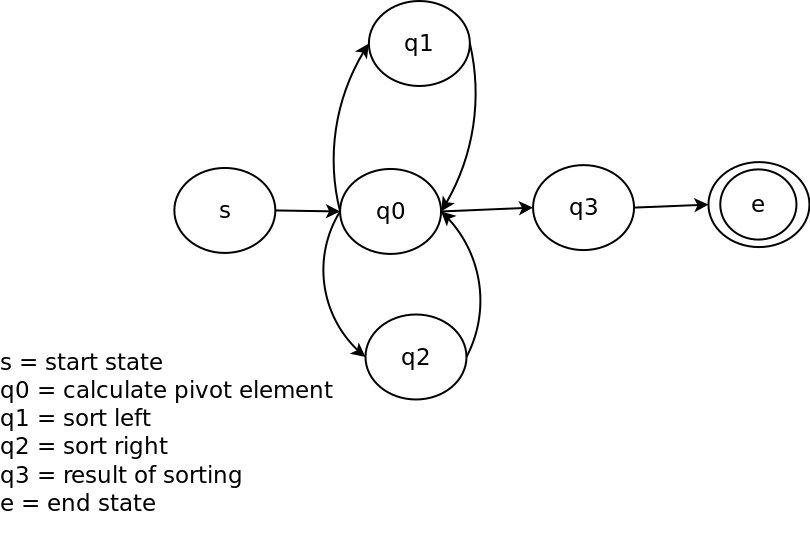
\includegraphics[scale=0.3]{stdg.png}


\section{Concepts related theory}
\subsection{Overview}
Quicksort (sometimes called partition-exchange sort) is an efficient sorting algorithm, serving as a systematic method for placing the elements of an array in order. Developed by Tony Hoare in 1959,[1] with his work published in 1961,[2] it is still a commonly used algorithm for sorting. When implemented well, it can be about two or three times faster than its main competitors, merge sort and heapsort.[3]

Quicksort is a comparison sort, meaning that it can sort items of any type for which a "less-than" relation (formally, a total order) is defined. In efficient implementations it is not a stable sort, meaning that the relative order of equal sort items is not preserved. Quicksort can operate in-place on an array, requiring small additional amounts of memory to perform the sorting.

Mathematical analysis of quicksort shows that, on average, the algorithm takes O(n log n) comparisons to sort n items. In the worst case, it makes O(n2) comparisons, though this behavior is rare.

\subsection{History}
The quicksort algorithm was developed in 1959 by Tony Hoare while in the Soviet Union, as a visiting student at Moscow State University. At that time, Hoare worked in a project on machine translation for the National Physical Laboratory. As a part of the translation process, he needed to sort the words of Russian sentences prior to looking them up in a Russian-English dictionary which was already sorted in alphabetic order on magnetic tape.[4] After recognizing that his first idea, insertion sort, would be slow, he quickly came up with a new idea that was Quicksort. He wrote a program in Mercury Autocode for the partition but couldn't write the program to account for the list of unsorted segments. On return to England, he was asked to write code for Shellsort as part of his new job. Hoare mentioned to his boss that he knew of a faster algorithm and his boss bet sixpence that he didn't. His boss ultimately accepted that he had lost the bet. Later, Hoare learned about ALGOL and its ability to do recursion which enabled him to publish the code in ACM.[5][2][self-published source?]

Quicksort gained widespread adoption, appearing, for example, in Unix as the default library sort function. Hence, it lent its name to the C standard library function qsort[6] and in the reference implementation of Java.

Robert Sedgewick's Ph.D. thesis in 1975 is considered a milestone in the study of Quicksort where he resolved many open problems related to the analysis of various pivot selection schemes including Samplesort, adaptive partitioning by Van Emden[7] as well as derivation of expected number of comparisons and swaps.[6] Bentley and McIlroy incorporated various improvements for use in programming libraries, including a technique to deal with equal elements and a pivot scheme known as pseudomedian of nine, where a sample of 9 elements is divided into groups of 3 and then the median of the 3 medians from 3 groups is chosen.[6] Jon Bentley described another simpler and compact partitioning scheme in his book Programming Pearls that he attributed to Nico Lomuto. Later Bentley wrote that he used Hoare's version for years but never really understood it but Lomuto's version was simple enough to prove correct.[8] Bentley described Quicksort as the "most beautiful code I had ever written" in the same essay. Lomuto's partition scheme was also popularized by the textbook Introduction to Algorithms although it is inferior to Hoare's scheme because it does 3 times more swaps on average and degrades to O(n2) runtime when all elements are equal.[9]

In 2009, Vladimir Yaroslavskiy proposed the new dual pivot Quicksort implementation.[10] In the Java core library mailing lists, he initiated a discussion claiming his new algorithm to be superior to the runtime library's sorting method, which was at that time based on the widely used and carefully tuned variant of classic Quicksort by Bentley and McIlroy.[11] Yaroslavskiy's Quicksort has been chosen as the new default sorting algorithm in Oracle's Java 7 runtime library after extensive empirical performance tests.[12]

\subsection{Algorithm}
Quicksort is a divide and conquer algorithm. Quicksort first divides a large array into two smaller sub-arrays: the low elements and the high elements. Quicksort can then recursively sort the sub-arrays.

The steps are:
\begin{enumerate}
\item Pick an element, called a pivot, from the array.

\item Partitioning: reorder the array so that all elements with values less than the pivot come before the pivot, while all elements with values greater than the pivot come after it (equal values can go either way). After this partitioning, the pivot is in its final position. This is called the partition operation.

\item Recursively apply the above steps to the sub-array of elements with smaller values and separately to the sub-array of elements with greater values.
\end{enumerate}

The base case of the recursion is arrays of size zero or one, which never need to be sorted.

The pivot selection and partitioning steps can be done in several different ways; the choice of specific implementation schemes greatly affects the algorithm's performance.


\section{Use case diagram}
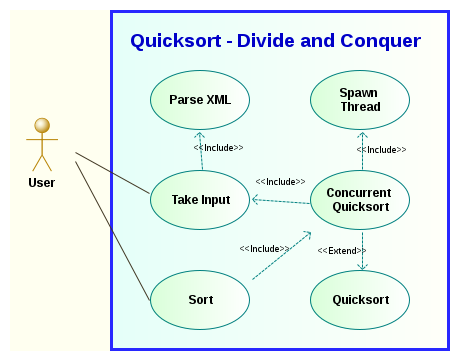
\includegraphics[scale=0.6]{use_case_diagram.png}


\section{Program Listing}
\begin{lstlisting}

------------ ConcurrentQuickSort.java ------------

public class ConcurrentQuicksort implements Runnable{

	int array[], lo, hi, id;
	public ConcurrentQuicksort(int array[], int lo, int hi, int id) {
		this.array = array;
		this.lo = lo;
		this.hi = hi;
		this.id = id;
	}
	public void quicksort() {
		if(lo<hi) {
			int p = partition();
			/*
			 * now spawn new threads here
			*/
			new Thread(new ConcurrentQuicksort(array, 
				lo, p-1, id*2)).start();
			new Thread(new ConcurrentQuicksort(array, 
				p+1, hi, id*2+1)).start();
		}
	}
	public int partition() {
		int pivot = array[hi];
		int i = lo;
		for(int j=lo; j<=hi-1; j++) {
			if(array[j]<=pivot) {
				swap(j,i);
				i++;
			}
		}
		swap(i,hi);
		return i;
	}
	public void swap(int x, int y) {
		if(x!=y) {
			int temp = array[x];
			array[x] = array[y];
			array[y] = temp;
		}
	}
	public String print(int lo, int hi) {
		String s = "array["+lo+".."+hi+"] = ";
		for(int i=lo; i<=hi; i++) {
			s += array[i]+ " ";
		}
		s+="\n";
		return s;
	}
	public void run() {
		System.out.print("Thread"+id+" is now" + 
			"sorting: "+print(lo,hi));
		quicksort();
	}
}


------------ InputParser.java ------------

import java.io.File;
import java.io.IOException;

import javax.xml.parsers.DocumentBuilder;
import javax.xml.parsers.DocumentBuilderFactory;
import javax.xml.parsers.ParserConfigurationException;

import org.w3c.dom.Document;
import org.w3c.dom.NodeList;
import org.xml.sax.SAXException;

public class InputParser {
	public int[] getInput() {
		int array[] = null;
		try {
			DocumentBuilderFactory dbFactory = 
				DocumentBuilderFactory.newInstance();
			DocumentBuilder dBuilder;
			dBuilder = dbFactory.newDocumentBuilder();
			File xmlFile = new File("src/input.xml");
			Document doc = dBuilder.parse(xmlFile);
			doc.getDocumentElement().normalize();
			NodeList nList = doc.getElementsByTagName("element");
			array = new int[nList.getLength()];
			for(int i=0; i<nList.getLength(); i++) {
				array[i] = 					
					Integer.parseInt(nList.item(i)
					.getTextContent());
			}
		} catch (ParserConfigurationException e) {
			// TODO Auto-generated catch block
			e.printStackTrace();
		} catch (SAXException e) {
			// TODO Auto-generated catch block
			e.printStackTrace();
		} catch (IOException e) {
			// TODO Auto-generated catch block
			e.printStackTrace();
		}
		return array;
	}
	public static void main(String args[]) {
		new InputParser();
	}
}

------------ TheMaster.java ------------

public class TheMaster {
	public static int mThreadCounter = 1;
	public static void main(String args[]) {
		TheWorker firstWorker = new TheWorker(mThreadCounter++);
		Thread t = new Thread(firstWorker);
		t.start();
	}
}

------------ TheWorker.java ------------


public class TheWorker implements Runnable{
	int id;
	public TheWorker(int n) {
		id = n;
	}
	public void run() {
		
		System.out.println("This is thread with id "+id);
		if(id>4) return;
		int left = id*2;
		int right = id*2+1;
		System.out.println(id+ " is now spawning" +
			"+left+" and "+right);
		new Thread(new TheWorker(left)).start();
		new Thread(new TheWorker(right)).start();
		
	}

}

------------ QuickSort.java ------------

public class Quicksort {

	public static void main(String[] args) throws InterruptedException {
		System.out.println("Enter the array to be" + 
			" sorted(space separated): ");
		InputParser parser = new InputParser();
		int array[] = parser.getInput();
		
		ConcurrentQuicksort qs = 
		new ConcurrentQuicksort(array, 0, array.length-1, 1);
		new Thread(qs).start();
		Thread.sleep(1000);
		
		// too lazy to use join or other methods to 
		// wait for all the threads to complete
		
		System.out.println("\nThe sorted array is:");
		for(int i=0; i<array.length; i++) {
			System.out.print(array[i]+ " ");
		}
		System.out.println();
	}
}

------------ Input.xml ------------

<?xml version="1.0"?>
<input>
	<array>
		<element>3</element>
		<element>1</element>
		<element>2</element>
		<element>7</element>
		<element>5</element>
		<element>6</element>
		<element>4</element>
	</array>
</input>

\end{lstlisting}


\section{Output}
\begin{lstlisting}

Enter the array to be sorted(space separated): 
3 1 2 7 5 6 4
Thread1 is now sorting: array[0..6] = 3 1 2 7 5 6 4 
Thread2 is now sorting: array[0..2] = 3 1 2 
Thread3 is now sorting: array[4..6] = 5 6 7 
Thread4 is now sorting: array[0..0] = 1 
Thread5 is now sorting: array[2..2] = 3 
Thread6 is now sorting: array[4..5] = 5 6 
Thread7 is now sorting: array[7..6] = 
Thread13 is now sorting: array[6..5] = 
Thread12 is now sorting: array[4..4] = 5 

The sorted array is:
1 2 3 4 5 6 7 

\end{lstlisting}


\section{Testing}
\subsection{White Box Testing}

\begin{figure}[h!]
	\centering
	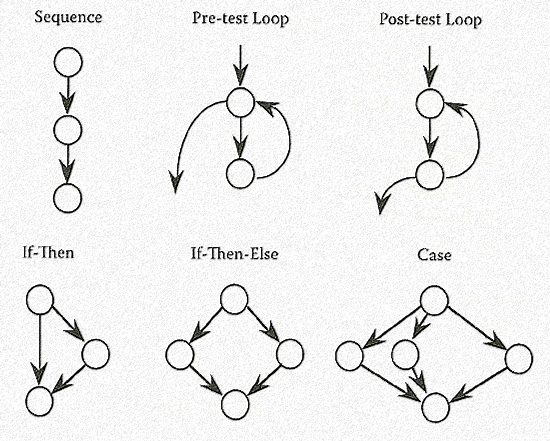
\includegraphics[scale=0.40]{flowgraph.png}
	\caption{Flow Graph Notation}
	\label{Flow Graph Notation}
\end{figure}


\begin{figure}[h!]
	\centering
	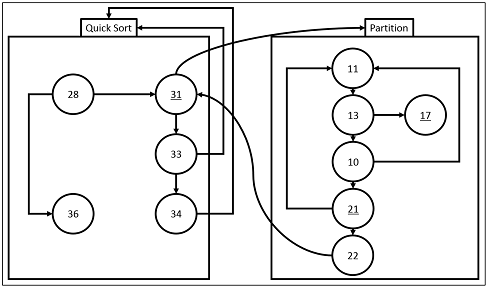
\includegraphics[scale=0.80]{graph.png}
	\caption{Flow Graph}
	\label{Flow Graph}
\end{figure}


\subsection{Positive Negative Testing}
\textbf{Example:}\\
Sample Input: For integer array\\
int A[] = f21; 33; 67; 72; 27; 10; 2; 66; 81; 1g; Function is passed following arguments:\\
quickSort(A; 0; 9);\\
Output obtained:\\
New partition: Low=0 High=9\\
Swapped 21 with Pivot 1\\
New partition: Low=1 High=9\\
Swapped 33 with 10\\
Swapped 67 with 2\\
Swapped 72 with Pivot 21\\
New partition: Low=1 High=2\\
Swapped 10 with Pivot 2\\
New partition: Low=4 High=9\\
Swapped 27 with 27\\
Swapped 33 with 33\\
Swapped 67 with 67\\
Swapped 66 with 66\\
Swapped 81 with Pivot 72\\
New partition: Low=4 High=7\\
Swapped 27 with 27\\
Swapped 33 with 33\\
Swapped 67 with Pivot 66\\
New partition: Low=4 High=5\\
Swapped 27 with 27\\
Swapped 33 with Pivot 33\\
1,2,10,21,27,33,66,67,72,81,\\
Note:\\
The underlined nodes are the ones being tested. The above output shows that every test region is
covered for given input.\\

\textbf{Positive Testing :}\\
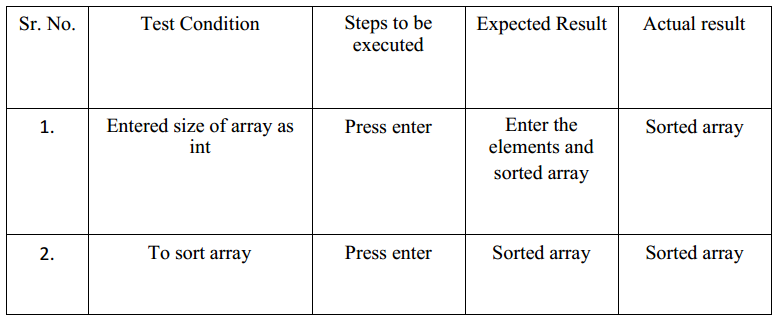
\includegraphics[width=\textwidth]{quicksort_positive}
\vspace{30px}

\textbf{Negative Testing :}\\
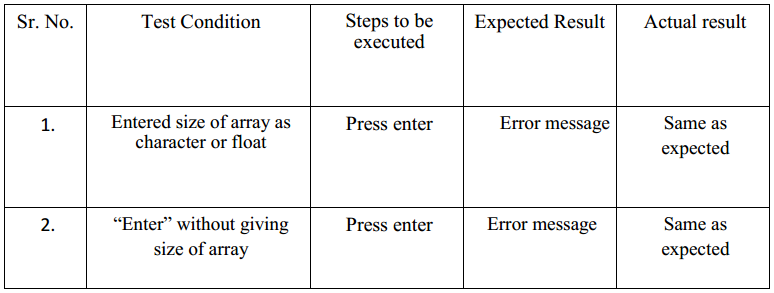
\includegraphics[width=\textwidth]{quicksort_negative}

\section{Conclusion}
Thus we have studied Quick Sort and implemented it using parallel framework of Threads in java. We have also acquired an acute sense of syntheiszing the documentation of typical softwares created in the industry.

\end{document}